\documentclass[11pt,letterpaper,boxed]{hmcpset}
\usepackage{fullpage}
\setlength{\parskip}{6pt}
\setlength{\parindent}{0pt}
\usepackage[margin=1in]{geometry}
\usepackage{graphicx}
\usepackage{enumerate}
\usepackage{marvosym}
\usepackage{amssymb}
\usepackage{wasysym}
\usepackage{gensymb}
\usepackage{mathrsfs}
\usepackage{scrextend}
\usepackage{mathtools}
\usepackage{pgfplots}
\usepackage{xspace}
\usepackage[colorlinks]{hyperref}

\makeatletter
\renewcommand*\env@matrix[1][*\c@MaxMatrixCols c]{%
   \hskip -\arraycolsep
   \let\@ifnextchar\new@ifnextchar
   \array{#1}}
\makeatother

% --- style --- %
\renewcommand{\labelenumi}{{ (\alph{enumi})}}
\newcommand{\sand}{\quad \mbox{ and } \quad}
%\newcommand{\ds}{\displaystyle}
\allowdisplaybreaks

% --- making \xi look less awful --- %
\DeclareSymbolFont{CMletters}{OML}{cmm}{m}{it}
\DeclareMathSymbol{\xi}{\mathord}{CMletters}{"18}

% --- math --- %
\newcommand{\Z}{\mathbb{Z}}
\newcommand{\R}{\mathbb{R}}
\newcommand{\C}{\mathbb{C}}
\newcommand{\Q}{\mathbb{Q}}


\newcommand{\Lt}[1]{\mathcal{L}\crb{#1}}
\newcommand{\ilt}[1]{\mathcal{L}^{-1}\crb{#1}}

\newcommand{\pn}[1]{\left( #1 \right)}
\newcommand{\sqb}[1]{\left[ #1 \right]}
\newcommand{\crb}[1]{\left\{ #1 \right\}}
\newcommand{\lra}[1]{\left\langle #1 \right\rangle}
\newcommand{\magn}[1]{\left\lVert #1 \right\rVert}

\newcommand{\pdr}[2]{\frac{\partial #1}{\partial #2}}
\newcommand{\im}[1]{\text{im}\pn{#1}}
\newcommand{\m}[1]{\Z/#1\Z}

\newcommand{\VEC}[1]{\ensuremath{\mathbf{#1}}\xspace}
\DeclareMathOperator{\proj}{proj}
\newcommand{\vectorproj}[2][]{\proj_{\VEC{#1}}\VEC{#2}}

\newenvironment{amatrix}[1]{%
  \left(\begin{array}{@{}*{#1}{c}|c@{}}
}{%
  \end{array}\right)
}

\makeatletter
\renewcommand*\env@matrix[1][*\c@MaxMatrixCols c]{%
  \hskip -\arraycolsep
  \let\@ifnextchar\new@ifnextchar
  \array{#1}}
\makeatother

\newcommand{\spn}[1]{\text{span}\pn{#1}}

\newcommand*\Heq{\ensuremath{\overset{\kern2pt H}{=}}}

\name{Box \#$\rule{1cm}{0.15mm}$}
\class{Math 60 Section 1}
\assignment{Homework 8}
\duedate{24 May 2018}

\begin{document}

%\begin{center}
\noindent\textbf{Collaborators:} 
%\end{center} 

%\problemlist{}

\begin{problem}[Colley 4.3 \#24]
You are sending a birthday present to your calculus instructor. Fly-By-Night Delivery Service insists that any package it ships be such that the sum of the length plus the girth be at most 108 in. (The girth is the perimeter of the cross section perpendicular to the length axis --- see Figure 4.31.) What are the dimensions of the largest present you can send?
\begin{center}
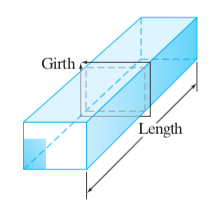
\includegraphics[scale=0.5]{prob1.png}
\end{center}
\end{problem}

\begin{solution}
\vfill
\end{solution}
\newpage

\begin{problem}[Colley 4.3 \#26]
An industrious farmer is designing a silo to hold her
$900\pi \text{ft}^3$ supply of grain. The silo is to be cylindrical in shape with a hemispherical roof. (See Figure 4.32.) Suppose that it costs five times as much (per square foot of sheet metal used) to fashion the roof of the silo as it does to make the circular floor and twice as much to make the cylindrical walls as the floor. If you were to act as consultant for this project, what dimensions would you recommend so that the total cost would be a minimum? On what do you base your recommendation? (Assume that the entire silo can be filled with grain.)
\begin{center}
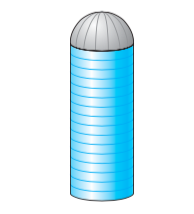
\includegraphics[scale=0.5]{prob2.png}
\end{center}
\end{problem}

\begin{solution}
\vfill
\end{solution}
\newpage

\begin{problem}[Colley 5.2 \#7]
Evaluate
\[
	\int_{-1}^3 \int_x^{2x+1}xy\,dy\,dx.
\]
In addition, sketch the region $D$ that is determined by the limits of integration.
\end{problem}

\begin{solution}
\vfill
\end{solution}
\newpage

\begin{problem}[Colley 5.2 \#14]
The following figure shows the level curves indicating varying depths (in feet) of a 25 ft by 50 ft swimming pool. Use a Riemann sum to estimate, to the 
nearest $100 \text{ft}^3$, the volume of water that the pool contains.
\begin{center}
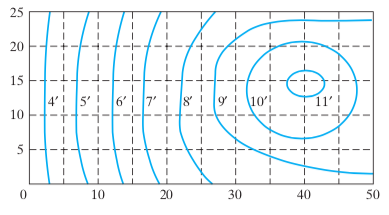
\includegraphics[scale=0.65]{prob3.png}
\end{center}
\end{problem}

\begin{solution}
\vfill
\end{solution}
\newpage

\begin{problem}[Colley 5.3 \#1]
Consider the integral
\[
	\int_0^2\int_{x^2}^{2x}(2x+1)\,dy\,dx.
\]
\begin{enumerate}
\item Evaluate this integral.
\item Sketch the region of integration.
\item Write an equivalent iterated integral with the order of integration reversed. Evaluate this new integral and check that your answer agrees with part (a).
\end{enumerate}
\end{problem}

\begin{solution}
\vfill
\end{solution}
\newpage

\begin{problem}[Colley 5.3 \#13]
Rewrite
\[
	\int_0^8\int_0^{\sqrt{y/3}}y\,dx\,dy+\int_8^{12}\int_{\sqrt{y-8}}^{\sqrt{y/3}}y\,dx\,dy
\]
as a single iterated integral by reversing the order of integration, and evaluate.
\end{problem}

\begin{solution}
\vfill
\end{solution}
\newpage

\begin{problem}[Colley 5.3 \#18]
Evaluate
\[
	\int_0^2\int_{y/2}^1e^{-x^2}\,dx\,dy.
\]
\end{problem}

\begin{solution}
\vfill
\end{solution}


\end{document}